% !TeX root = ../thuthesis-example.tex

\chapter{基于弹性张量的大模型微调内存优化}

\section{概述}

大语言模型\cite{GPT-3,llama2,bloom176b,gpt4}正日益普及。
与此同时,个性化以及支持个性化的微调技术\cite{sun2019fine,wortsman2022robust,dodge2020fine}已成为大模型后训练领域的热门研究话题。
微调通常在有限的数据和典型的硬件配置下完成\cite{zhou2023mpress,feng2023mobius,atc-finetune},并且需要快速生成多个微调模型 ~\cite{ftsurvey-1,ftsurvey-2,ftsurvey-3}。
然而,由于大语言模型参数数量巨大,进行全参数微调难以满足上述要求 ~\cite{zhou2022pets,slora,opendelta}。

为解决这一问题,研究人员提出了参数高效微调(Parameter-Efficient Fine-Tuning, PEFT)。
与全参数微调不同,PEFT 从大模型的预训练权重出发,仅训练一小部分权重,同时冻结大部分权重\cite{peft-adapter-lora,peft-prompt-tuning,peft-adapterfusion,peft-bitfit,peft-P-tuning}。
这大幅减少了训练模型的计算量和存储需求(因为只需存储训练的那部分权重),同时仍能实现理想的模型性能。因此,PEFT 现已成为微调的主流方法\cite{peft-overview,delta-tuning-overview,opendelta}。

在微调过程中,每个设备存储模型权重以及训练过程中生成的中间结果(激活值)。权重和激活值的大小与模型规模相关,大型模型的参数规模可达数十亿甚至数百亿。然而,单个 GPU 的内存限制通常仅为几十 GB。因此,权重和激活值需要在多个设备间进行划分,由此产生的通信开销成为性能瓶颈~\cite{zhou2023mpress,feng2023mobius}。

\begin{figure}[ht]
     \centering
     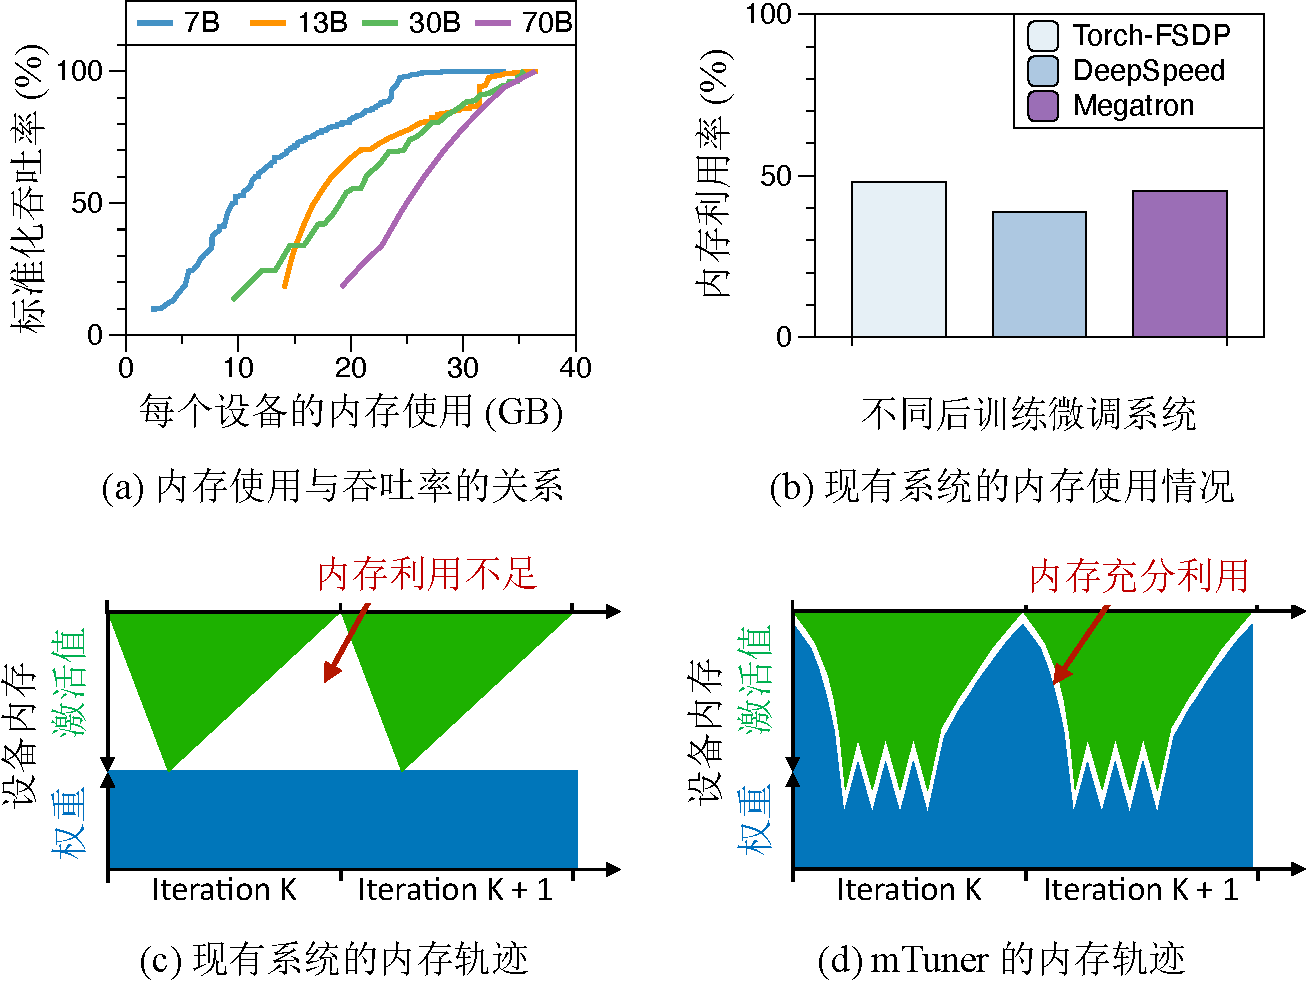
\includegraphics[width=0.8\textwidth]{figures/mtuner/intro-crop.pdf}
     % \begin{subfigure}[b]{0.35\textwidth}
     %     \centering
     %     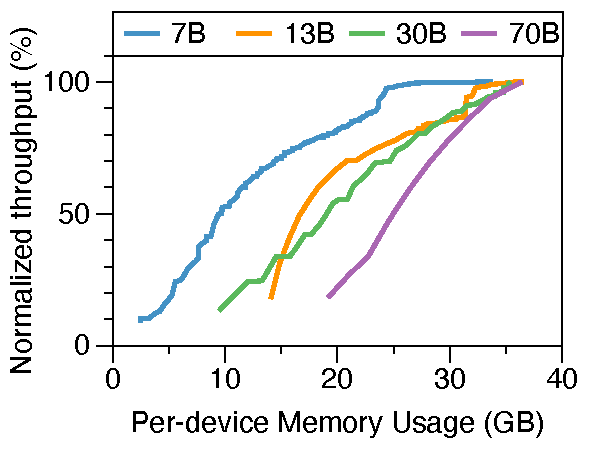
\includegraphics[width=\textwidth]{figures/mtuner/intro-mem-tput.pdf}
     %     \caption{}
     %     \label{fig:intro-mem-tput}
     % \end{subfigure}
     % % \hfill
     % \begin{subfigure}[b]{0.35\textwidth}
     %     \centering
     %     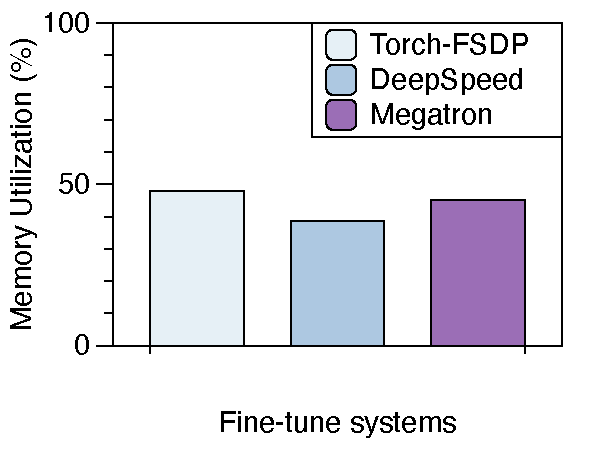
\includegraphics[width=\textwidth]{figures/mtuner/intro-mem-usage.pdf}
     %     \caption{}
     %     \label{fig:intro-mem-usage}
     % \end{subfigure}
     % \vfill
     % \begin{subfigure}[b]{0.35\textwidth}
     %     \centering
     %     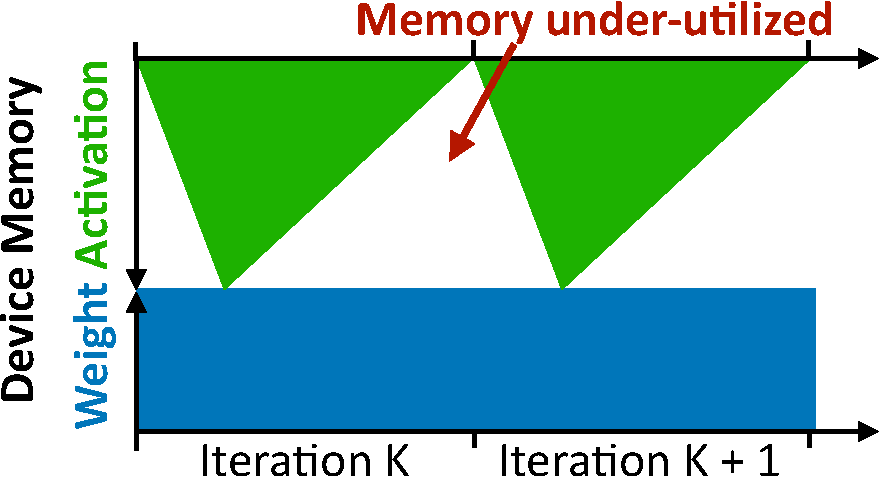
\includegraphics[width=\textwidth]{figures/mtuner/intro1-crop.pdf}
     %     \caption{}
     %     \label{fig:intro-c13}
     % \end{subfigure}
     % % \hfill
     % \begin{subfigure}[b]{0.35\textwidth}
     %     \centering
     %     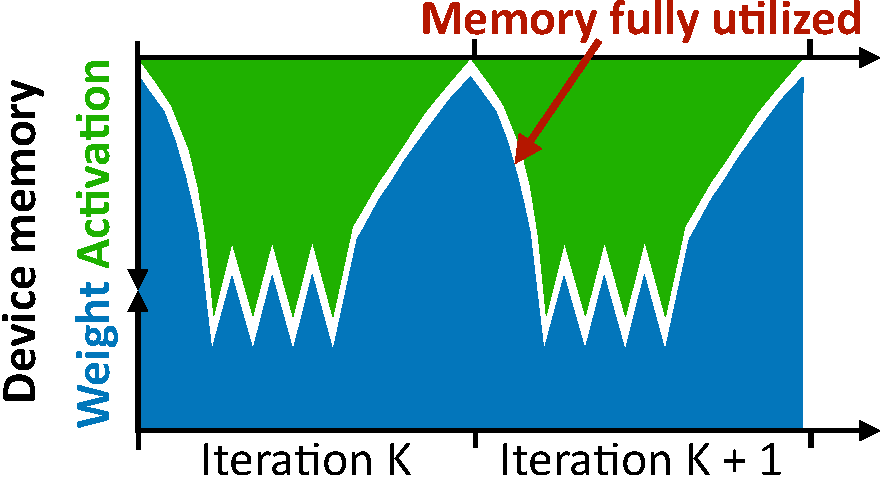
\includegraphics[width=\textwidth]{figures/mtuner/intro2-crop.pdf}
     %     \caption{}
     %     \label{fig:intro-c2}
     % \end{subfigure}
     % \hfill
     % \begin{subfigure}[b]{0.23\textwidth}
     %     \centering
     %     \includegraphics[width=\textwidth]{img/challenge2-crop.pdf}
     %     \caption{}
     %     \label{fig:intro-c2}
     % \end{subfigure}
        \caption{
        后训练微调内存优化的研究动机
        % (a) The overall throughput is 
        % Device memory usage for fine-tuning of previous works (a) and mTuner (b)
        }
        \label{fig:mtuner-intro}
\end{figure}


经测试,本研究发现在微调过程中,内存资源利用率不高。而在该场景中,利用空闲内存恰好可以有效优化通信,这对后训练的整体性能提升至关重要。
具体地,对于权重而言,更多的本地可用权重可以减少后训练过程中的通信量;
对于激活值,使用更大的批量大小虽然会增加激活值的内存需求,但可以降低每个样本的通信量。
如\Cref{fig:mtuner-intro}(a)所示,随着内存使用量的增加,不同模型的吞吐量能够得到显著提升。

现有工作已经尝试利用内存优化提升预训练性能。
Deepspeed~\cite{rasley2020DeepSpeed} 和 Torch-FSDP~\cite{TorchFSDP}采用数据并行和零冗余优化(ZeRO)方法,为每个设备分配一部分样本。
Megatron~\cite{krothikanti2022megatronv3}  集成了数据并行、张量并行和流水线并行,对模型权重进行划分以减少通信开销。
然而,如\Cref{fig:mtuner-intro}(b)所示,在后训练PEFT微调场景中,现有工作的平均内存利用率较低。
本研究总结以下两个原因:

\begin{itemize}
    \item 
    \textbf{激活值的峰谷模式}:
    由于微调过程中反向传播的特性,在前向传播阶段首先生成的激活值直到反向传播的最后阶段才会被使用和释放。
    如\Cref{fig:mtuner-intro}(c)所示,这种先进后出(FILO)的工作流程导致激活值内存使用呈现峰谷模式,造成大量内存未被充分利用(白色部分)。
    \item 
    \textbf{静态划分的权重}:
    激活值的内存使用在运行时动态变化,而权重在训练前被静态划分,并且在训练过程中不会进行调整。
    这种限制使得权重无法根据当前内存使用情况及其变化趋势进行动态调整。
    如\Cref{fig:mtuner-intro}(c)所示,静态划分的权重无法利用激活值在低谷区域留下的内存空间。
\end{itemize}

经观察,在 PEFT 中,权重和激活值的内存都可以进行动态高效的调整:对于 PEFT 中的权重,由于大部分权重被冻结,在不同设备上复制这些权重不会引入额外的同步开销。
同时,通过细粒度地改变计算执行顺序,可以灵活修改驻留在内存中的激活值的大小和生命周期。

基于此观察,本研究提出弹性张量的概念,以统一权重和激活值的动态内存管理。
张量(权重和激活值)的大小在运行时动态调整,使权重内存和激活值内存之间的权衡适应当前内存使用情况和后训练微调过程。
在收集完整权重进行计算时调整权重内存,并通过细粒度地生成、保存检查点和消耗激活值,灵活确定激活值的生命周期,从而调整其内存使用量。
如\Cref{fig:mtuner-intro}(d)所示,权重可以填充激活值内存的低谷区域,减少通信量;激活值可以降低峰值内存使用量,保持较高的内存利用率。

基于弹性张量,本章构建了一个具有高内存利用率的微调系统 mTuner,可提高后训练 PEFT 微调效率。
mTuner 在运行时利用弹性权重和激活值,实现高内存利用率以节省通信量。
在配备8个 GPU 的服务器上,对基于 Transformer、参数规模从 70 亿到 700 亿的大语言模型进行评估。
实验结果表明,与 Deepspeed ~\cite{rasley2020DeepSpeed} 和 Megatron ~\cite{krothikanti2022megatronv3} 等最先进的训练系统相比,mTuner 可将微调性能提升最高达 1.51 倍(平均提升 1.28 倍)。
mTuner 的吞吐量超过每秒 30,000 个词元,并且能够在 3 小时内使用 Llama-2-13B 模型对数学数据集 ~\cite{math-datatset}  进行微调。

本章研究的主要贡献如下:

1. 对后训练 PEFT 微调的内存使用情况进行了详细分析,揭示了内存使用率不足的原因;

2. 提出了弹性张量,能够灵活动态地调整权重和激活值的内存使用量;

3. 基于弹性张量构建 mTuner,使执行计划能够适应内存状态,实现高效微调;

4. 在参数规模从 70 亿到 700 亿的各种大语言模型上对 mTuner 进行评估,在 PCIe GPU 服务器上实现了最高 1.51 倍(平均 1.28 倍)的吞吐量提升,并且能够在 3 小时内微调模型以适应特定领域。

\section{研究动机}

\subsection{权重与并行训练}
在大语言模型中,每个权重都与一个算子相关联,为了对该算子进行前向或后向计算,需要完整的权重。
一个模型由大量算子组成,导致总权重规模巨大,参数数量从数十亿到数百亿不等。

因此,模型权重的大小通常超出了单个 GPU 的存储限制。
为了进行大型模型后训练,需要将模型权重分片存储在多个 GPU 上。
以配备8个 GPU 的服务器为例,每个 GPU 存储每个算子 12.5\%(1/8)的权重。
在前向传播过程中,当需要执行某个算子的计算时,GPU 之间通过全收集(allgather)操作相互通信,获取该算子的所有权重,然后使用完整权重对本地样本进行算子计算,并丢弃收集到的权重。
类似地,在反向传播过程中,也需要进行权重收集和丢弃操作。
因此,在一次迭代中,每个 GPU 的通信量是模型权重大小的两倍。
这就是全分片数据并行(FSDP)\cite{TorchFSDP}的工作流程,该方法常用于并行训练 \cite{rasley2020DeepSpeed,fan2021dapple}。

\subsection{激活值与运行时内存}
除了并行化方案分配的模型权重外,微调的内存开销还包括运行时生成的中间结果,即激活值。
这些激活值在前向传播过程中生成,用于梯度计算,并在反向传播过程中释放。
由于反向传播的特性,前向传播开始时产生的激活值在反向传播结束时才会被消耗。
这导致大量激活值驻留在内存中,形成明显的峰谷模式。
峰值出现在前向传播结束(反向传播开始)时,谷值出现在前向传播开始(反向传播结束)时。
激活值的总大小与批量大小、输入序列长度和模型大小有关,通常消耗大量内存。
例如,当输入序列长度为 1024 时,70 亿参数模型上每个样本生成的激活值约为 4GB,这与模型参数占用的总内存(14GB)相当。

\subsection{局限性分析}

(1) \textbf{内存利用率低下}:
具有峰谷特性的激活值内存利用率较低。
尽管在峰值时设备内存得到充分利用,但在其他时间存在未使用的内存,导致激活值内存平均闲置率达 50\%。
峰值的存在进一步限制了批量大小。
在用于微调的小规模硬件配置中,可实现的批量大小较小,导致计算并行度低,每个样本的通信开销较大。
此外,峰值高度与模型大小和输入序列长度呈正相关。
随着训练数据越来越倾向于长文本,激活值已成为更显著的内存开销。

(2) \textbf{缺乏灵活性}:
现有方法在后训练微调前确定权重的分布并将其划分到各个设备,该决策基于设备数量和总权重大小。
在微调过程中,权重占用的内存大小无法改变。
这种静态的权重内存分配方法无法感知运行时内存使用情况及其变化趋势,可能导致内存未充分利用或内存不足的情况。

(3) \textbf{忽视权重与激活值的相互作用}:
在训练过程中,权重和激活值共存于内存中,竞争内存资源。
此外,它们呈现出不同的内存模式:已分配的权重持续占用内存,而激活值呈现周期性的峰谷变化。
因此,它们之间的相互作用对于高效利用内存至关重要。
然而,现有方法分别独立优化权重的并行训练和激活值的运行时计划,无法实现同时考虑这两个方面系统性地寻找最优解决方案。

\begin{figure}[ht]
\centerline{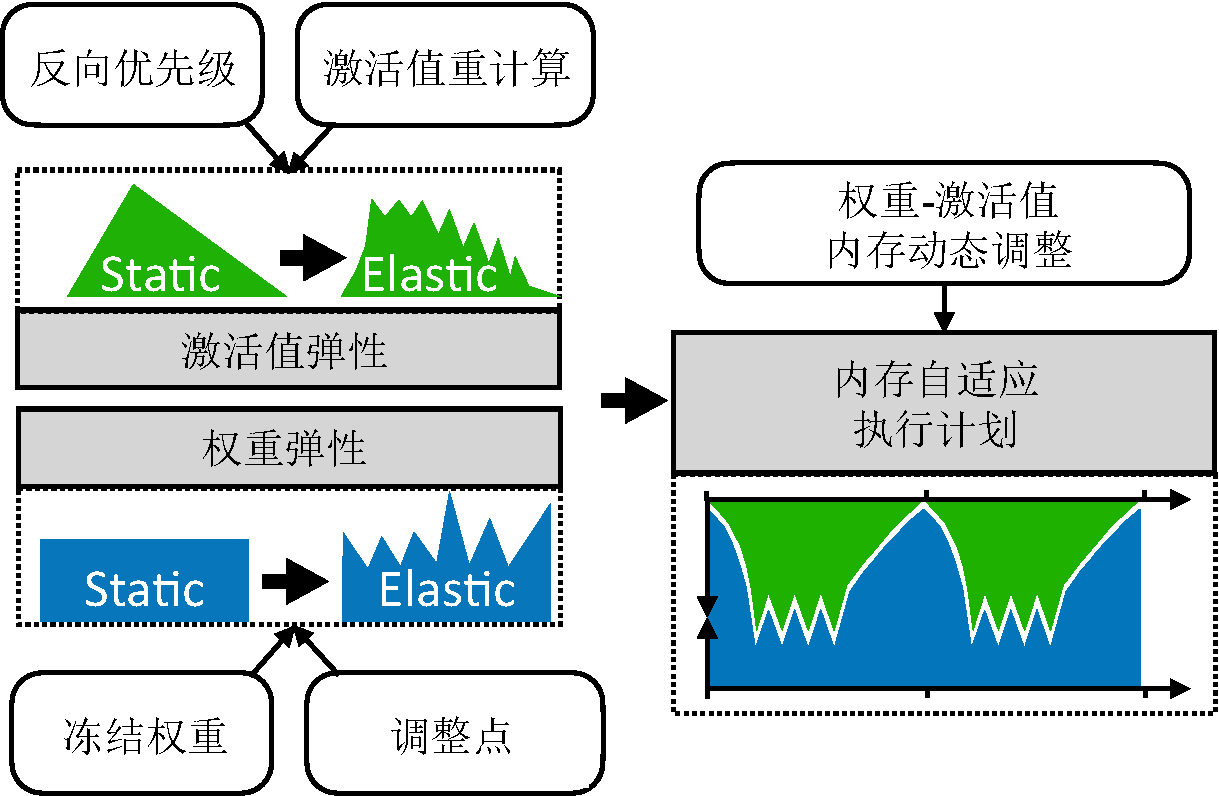
\includegraphics[width=0.6\textwidth]{figures/mtuner/overview-crop.pdf}}
\caption{mTuner系统设计}
\label{fig:mtuner-overview}
\end{figure}

\section{mTuner系统概述}
\Cref{fig:mtuner-overview}展示了 mTuner 的系统概述。
mTuner 的设计基于微调过程中张量的特殊属性--张量的弹性:权重和激活值张量的内存使用量都可以灵活动态地变化。
\Cref{mtuner:sec:elastic-tensor}将分别深入探讨权重和激活值的张量弹性,讨论改变它们大小的方法以及相关的成本和收益。
\Cref{mtuner:sec:training-plan}将探讨 mTuner 如何感知内存状态,并根据内存状态开发自适应内存的执行计划,利用张量弹性针对不同的内存状态进行优化,然后介绍 mTuner 如何根据硬件设置和模型结构搜索具体的执行计划。


\section{弹性张量}
\label{mtuner:sec:elastic-tensor}

在微调过程中,需要长时间驻留在内存中的张量会占用大量内存,这包括分配给设备的权重内存以及设备计算过程中生成的中间结果(激活值)。
本章研究发现,在 PEFT 的背景下,这些张量的内存大小可以进行调整。
通过各种方式,可以增加或减少权重和激活值的内存使用量,同时需要考虑执行成本和收益之间的权衡。

\subsection{权重弹性}

\subsubsection{冻结权重}

由于 PEFT 区分基础模型和适配器的设计,其大部分权重(来自基础模型的权重)在训练过程中不会被更新,这些权重被称为\textbf{冻结权重}。
尽管冻结权重不会更新,但它们仍然参与前向和后向计算(分别用于获取激活值和计算激活值的梯度)。
在传统的并行训练系统中,它们被视为普通权重。

然而,本研究发现由于这些冻结权重保持不变,它们可以在不同设备上冗余存储而不引入额外的同步开销。
也就是说,对于在 D 个设备上进行的分布式微调,每个设备上权重的存储比例可以从\(\frac{1}{D}\)(全分片)连续变化到 100\%(全复制)。
本研究将这些存储比例可连续变化的权重称为弹性权重。

\subsubsection{权重大小的动态调整}

如\Cref{fig:adjust-point}(a)和(b)所示,在执行一个算子时,每个设备通过通信(解分片,unshard)获取其完整权重,然后用于计算。
计算完成后,收集到的权重被释放(重新分片,reshard)。

由于设备在计算过程中拥有完整的权重,mTuner 可以在不产生额外通信开销的情况下重新调整权重大小。
在\Cref{fig:adjust-point}(c)的示例中,在计算前,每个设备仅拥有算子权重的\(\frac{1}{D}\),计算后调整为\(\frac{2}{D}\)。
这种动态调整可以在每次使用权重进行计算时进行,后文将这些时刻称为调整点。



\begin{figure}[ht]
\centerline{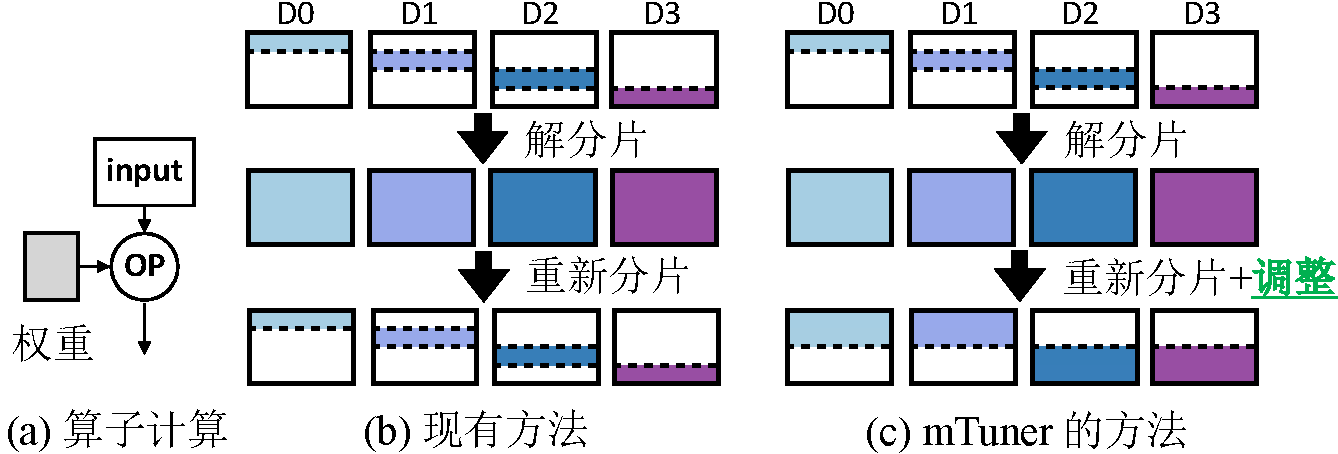
\includegraphics[width=0.65\textwidth]{figures/mtuner/adjust-point-crop.pdf}}
\caption{权重调整点的示意图}
\label{fig:adjust-point}
\end{figure}

在一次迭代中,每个算子的权重至少有两个调整点:前向计算时和反向计算时。
如果应用激活值检查点的重新计算,调整点可能会多于两个。
mTuner 可以在这些调整点动态改变权重大小,以适应不同的内存使用情况。

\subsubsection{弹性权重的搜索空间}

弹性权重的大小可以在两个维度上进行调整:算子内和算子间。
在算子内维度上,对于给定的算子,mTuner 可以将单个设备上存储的权重大小从\(\frac{1}{D}\)调整到 100\%。
然而,如果将弹性权重大小设置为\(\frac{k}{D}\),只有当 k 是 D 的因数时,才能缩小通信范围(从 D 个设备间的通信缩小到\(\frac{D}{k}\)个设备间的通信),从而显著提高通信效率。
因此,在算子内维度上,mTuner 仅在 k 是 D 的因数时将弹性权重大小设置为\(\frac{k}{D}\)。
例如,在使用8个 GPU 进行微调的情况下,每个算子的权重大小仅会选择 12.5\%、25\%、50\% 或 100\%。

尽管算子内维度的这种选择策略可能会限制权重大小的灵活性,但在算子间维度上,不同的算子可以独立选择不同的弹性权重大小。
由于大语言模型由大量算子组成,通过组合不同权重大小的算子,可以灵活配置整体弹性权重大小,使其连续覆盖从\(\frac{1}{D}\)到 100\% 的值。

\subsection{激活弹性}
在参数高效微调(PEFT)中,mTuner 还可以使激活具备弹性,以缓解因峰谷内存模式导致的内存利用率低下问题。
本研究发现,激活在内存中累积的主要原因是其先进后出(FILO)模式,以及由此产生的激活驻留时间长。
因此,mTuner 采用两种方法来缩短生成的激活的生命周期,从而减少 FILO 模式带来的问题。
第一种方法是提高反向计算的执行优先级,优先消耗前向传播过程中生成的激活;第二种方法是丢弃部分激活,并在反向传播过程中重新生成这些激活。

\subsubsection{提高反向计算优先级}
激活在前向传播阶段生成,在反向传播阶段使用并释放。
因此,更早地执行反向计算可以缩短生成的激活的生命周期,使其更早地释放,减少在内存中的驻留时间。
然而,在前向-反向计算范式中,必须先计算所有前向算子以获取损失,然后才能进行反向计算,这个顺序是不可改变的。
为了便于更早地执行反向计算,本研究提出沿样本维度拆分和重新排列计算顺序。

\begin{figure}[ht]
\centerline{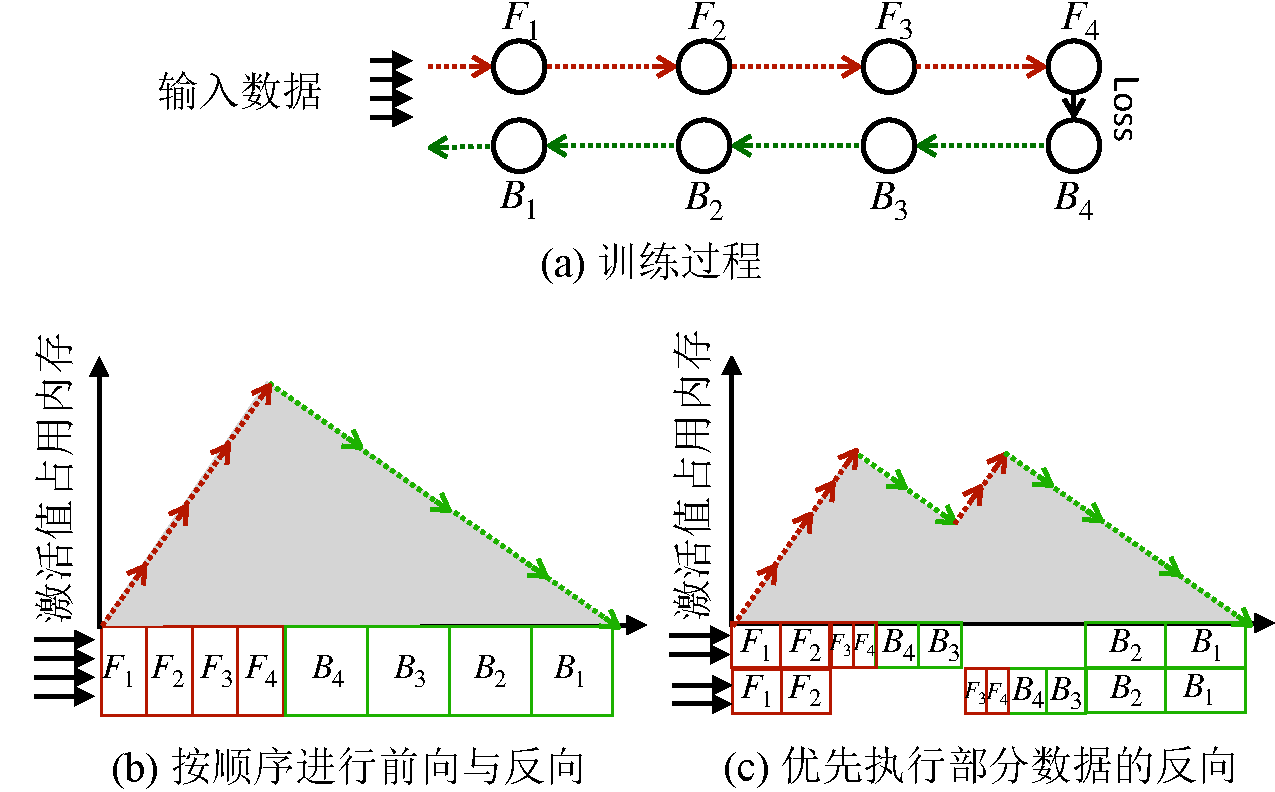
\includegraphics[width=0.68\textwidth]{figures/mtuner/backward-prior-crop.pdf}}
\caption{提高反向计算优先级示意图}
\label{fig:backward-prior}
\end{figure}

如\Cref{fig:backward-prior}(a)所示,对于在四个输入样本上训练一个 4 层模型,典型的过程是将它们一起处理,先执行四个前向计算,然后执行四个反向计算。
如\Cref{fig:backward-prior}(b)所示,这个过程导致四个样本在前向传播结束时生成的激活都驻留在内存中,直到反向传播开始。由于所有激活都累积起来,内存使用量达到峰值。
为了更早地释放激活,mTuner 将样本划分为更小的批次,每个批次包含一个或多个样本。
然后,对每个批次依次执行前向和反向计算,而不是将所有样本一起处理。
如\Cref{fig:backward-prior}(c)所示,对于四个样本的批次,mTuner 将它们分成两个批次,每个批次包含两个样本。
它先对第一个批次执行前向计算,然后执行反向计算,释放第一个批次生成的激活。
然后,对第二个批次重复相同的过程。通过这种方式,每个批次生成的激活在反向计算完成后立即释放,而不是累积到所有前向计算完成后,从而降低了峰值内存使用量。


% The height of the peak can be arbitrarily adjusted using this method. Let the total batch size be $B$, the batch size after splitting be $b$, and the model consists of $L$ layers. Among them, the $l$ layers closer to the peak adjust the backward priority. Suppose the original peak height is H, then the new peak height is calculated as:

% \begin{equation}
% H_{new} =   \frac{l}{L}  \frac{b}{B} H+   (1 - \frac{l}{L})H
% \end{equation}

% This formula indicates that as the ratio of $b$ to $B$ decreases, the height of the adjusted backward priority portion becomes lower. Additionally, as more layers are adjusted in terms of peak height, the final peak height will also be reduced. When $l=L$ and $b=1$, it is equivalent to running the entire model with a batch size of 1, resulting in the lowest peak height.


\subsubsection{激活值重计算}
除了重新排列计算顺序外,mTuner 还采用激活重计算技术进一步减少激活内存使用。
激活重计算是一种通过重新计算激活而不是将其存储在内存中来减少激活内存占用的方法。
在前向传播过程中,mTuner 不存储所有生成的激活,而是仅存储少量关键激活,这些关键激活足以在反向传播过程中重新计算其余激活。
在反向传播过程中,mTuner 使用存储的关键激活重新计算所需的激活,而不是从内存中读取它们。

如\Cref{fig:activation-checkpoint}所示,对于一个 4 层模型,mTuner 可以选择仅存储第 1 层和第 3 层的激活作为关键激活。
在反向传播过程中,当需要第 2 层的激活时,mTuner 使用存储的第 1 层激活重新计算第 2 层的激活。
通过这种方式,mTuner 可以显著减少激活内存使用,因为它只需要存储少量关键激活,而不是所有生成的激活。
然而,激活重计算也引入一些开销。
由于在反向传播过程中需要重新计算激活,这会增加计算时间。
因此,mTuner 需要在激活内存使用和计算时间之间进行权衡,以确定要存储的关键激活的最佳数量。

\begin{figure}[ht]
\centerline{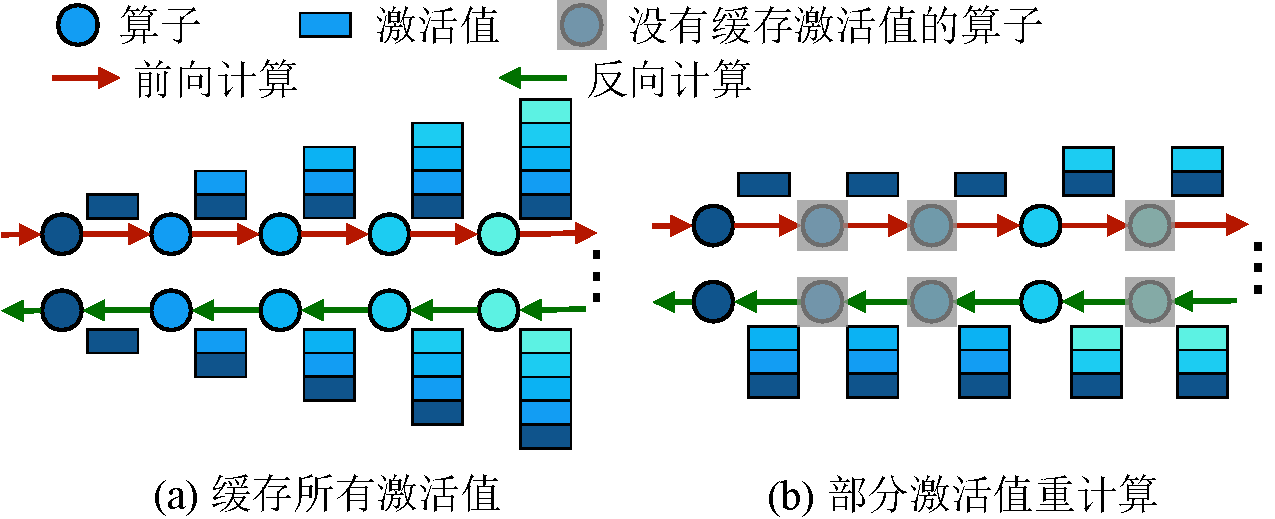
\includegraphics[width=0.68\textwidth]{figures/mtuner/activation-checkpoint-crop.pdf}}
\caption{激活值重计算示意图}
\label{fig:activation-checkpoint}
\end{figure}


\subsubsection{激活弹性的搜索空间}
激活弹性的大小可以在两个维度上进行调整:样本维度和层维度。

在样本维度上,mTuner 可以调整批次大小,即将样本划分为不同大小的批次。
较小的批次大小可以更早地释放激活,降低峰值内存使用量,但会增加计算开销,因为每个批次都需要单独的前向和反向计算。
较大的批次大小可以减少计算开销,但会增加峰值内存使用量。
因此,mTuner 需要根据可用内存和计算资源在样本维度上选择合适的批次大小。

在层维度上,mTuner 可以选择存储哪些层的激活作为关键激活。
不同的层选择会导致不同的激活内存使用和计算时间。
存储更多层的激活作为关键激活可以减少反向传播过程中的计算时间,但会增加激活内存使用。
存储较少层的激活作为关键激活可以减少激活内存使用,但会增加反向传播过程中的计算时间。
因此,mTuner 需要在层维度上找到激活内存使用和计算时间之间的最佳平衡。

\section{内存自适应执行计划}
\label{mtuner:sec:training-plan}

在\Cref{mtuner:sec:elastic-tensor}中,本研究讨论了权重和激活的弹性,以及它们在内存使用方面的动态调整能力。
本节主要介绍 mTuner 如何利用这些弹性张量来制定自适应内存执行计划,以适应不同的内存状态并优化微调性能。
首先,本节分析训练过程中的内存状态,提出了\textit{内存阶段}和\textit{重用距离}的概念,这些概念能有效刻画后训练微调过程中的内存状态,帮助识别内存重用的机会。
随后,本节展示了如何在内存状态的引导下,利用弹性张量使执行计划适应内存情况。
最后,本节介绍 mTuner 如何在给定硬件设置和模型结构的情况下搜索执行计划。

\subsection{内存阶段与重用距离}

(1) {\textbf{内存阶段}}:
运行时激活值的先进后出模式导致激活内存出现峰值和谷值,将训练过程划分为不同的内存阶段。
在峰值区域,内存极其稀缺,需要节省内存的执行计划;而在谷值区域,内存充足,可以探索以空间换时间的优化技术。
这些区域对内存自适应优化至关重要。

\begin{figure}[ht]
\centerline{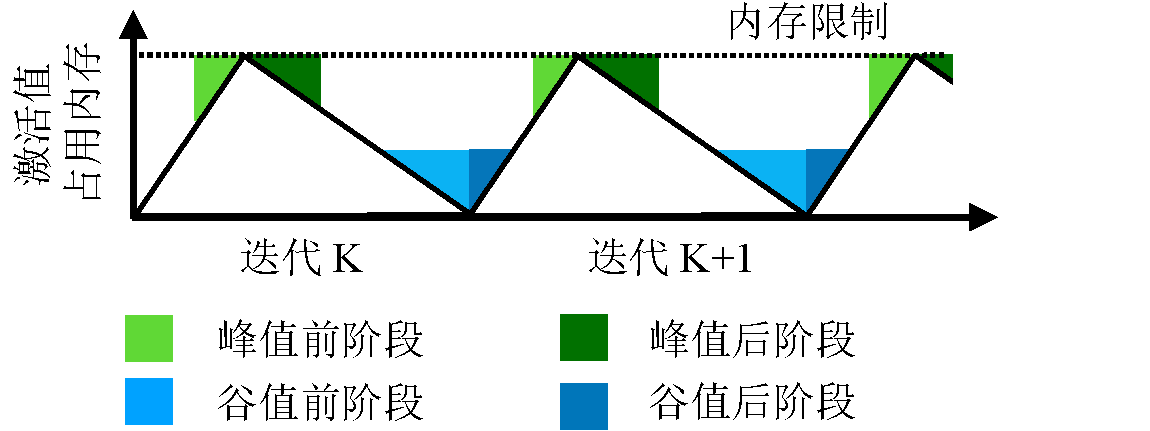
\includegraphics[width=0.62\textwidth]{figures/mtuner/memory-stage-crop.pdf}}
\caption{运行时生成的激活值导致的内存阶段}
\label{fig:memory-stage}
\end{figure}

因此,本研究基于与这些峰值和谷值的关系来定义内存阶段,考虑两个方面:与峰值/谷值的距离,以及处于峰值/谷值之前还是之后。
在\Cref{fig:memory-stage}中,以峰值为例,与峰值的距离决定了当前的内存剩余量,在一次迭代中,离峰值越远,内存越充足。
峰值前后的关系决定了当前内存使用的变化:在峰值之前,内存消耗持续增加,无法存储额外数据;在峰值之后,内存使用稳步减少,为存储额外数据以供重用提供了机会。
谷值的情况则完全相反。

(2) {\textbf{重用距离}}:
重用距离是内存利用率的另一个重要因素,它指的是同一张量当前使用与下次重用之间的间隔长度。
本研究观察发现,在峰值前阶段,权重和激活值的重用距离都很小。
这是因为在靠近损失计算的模型部分,前向计算之后立即进行相应的反向计算,使得峰值前阶段使用的张量能在峰值后阶段及时重用。
谷值前阶段的情况类似,在谷值前阶段,冻结的权重由于不需要更新,可以在谷值后阶段的前向计算中重用。
然而,谷值后阶段的激活值是新生成的,无法重用谷值前阶段的激活值。

重用距离可以指导内存自适应执行计划。
对于重用距离小的张量,增加其在内存中的弹性大小有利于即将进行的数据重用;对于重用距离大的张量,减小其弹性大小可以为其他张量腾出空间。

\subsection{基于峰谷感知的内存优化}

从上述分析可知,峰值和谷值区域在内存利用率和数据重用方面都存在显著的优化潜力。
因此,mTuner 针对这两个区域进行了专门的优化。

\subsubsection{渐进填充谷值区域}

在谷值区域,谷值前阶段的冻结权重具有极小的重用距离。
因此,mTuner 会在谷值前的调整点增加弹性权重的大小,使这些弹性权重能在谷值后阶段的前向计算中被重用,并在谷值后阶段的调整点将弹性权重调整回基准值。由于该操作发生在激活内存占用较低时,存储这些弹性权重不会产生额外开销。

\begin{figure}[ht]
\centerline{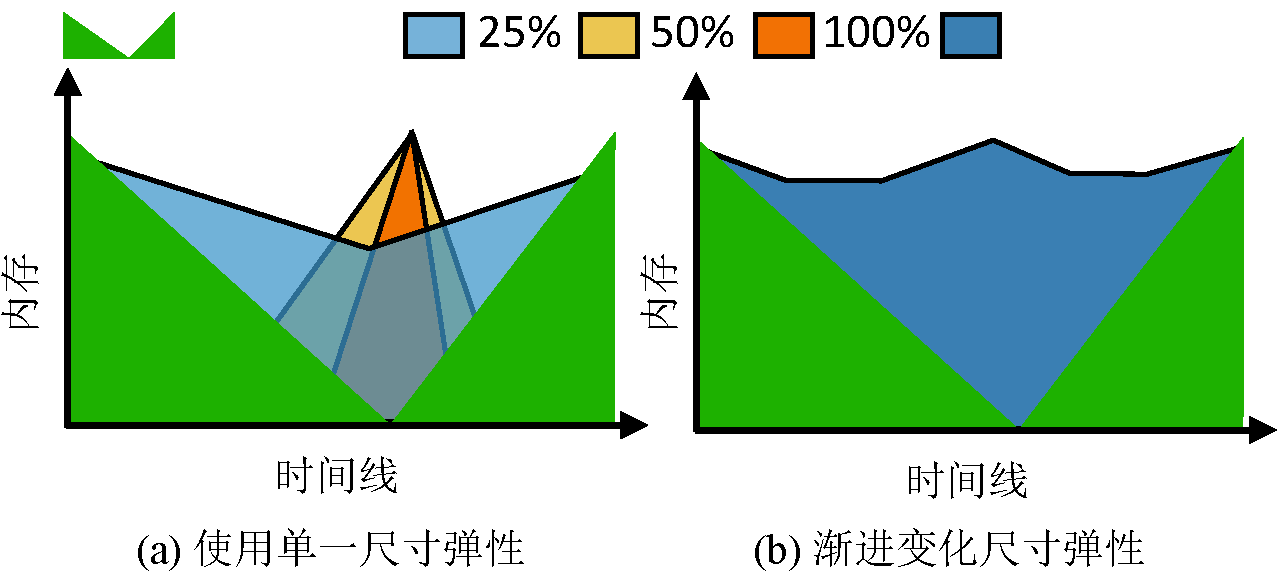
\includegraphics[width=0.68\textwidth]{figures/mtuner/progressive-crop.pdf}}
\caption{不同策略下弹性权重填充内存示意图}
\label{fig:progressive}
\end{figure}

此外,本研究观察到越靠近谷值的位置,可用空闲内存越多,允许在此处使用更高比例的弹性权重(如高达100\%)。
相反,离谷值较远的位置由于靠近峰值且受设备内存限制,应使用较低比例的弹性权重。
因此,在谷值前区域,弹性权重的存储比例随与谷值距离的减小而增加。  
因此,mTuner 并非使用单一弹性权重尺寸,而是渐进采用不同大小的弹性权重,以最大化谷值区域的空闲内存利用率。
如\Cref{fig:progressive}所示,(a)展示了用单一尺寸弹性权重填充谷值的情况:若使用较大弹性权重(50\%或100\%),谷值会被快速填满,但其他区域仍有大量内存未被使用;若使用较小弹性权重(25\%),则谷值无法被填满。
(b)则通过不同尺寸弹性权重渐进填充谷值,实现了更高的内存利用率。

\subsubsection{展平峰值高度}

弹性激活值可通过改变峰值区域算子的反向计算优先级,有效降低峰值高度。mTuner 可利用降低后的峰值高度,在非峰值位置增加批量大小或增大弹性权重尺寸。  
但本研究发现,改变峰值高度后,峰值区域的计算需要对不同样本执行$\frac{B}{b}$次,这导致峰值区域的权重需被多次完整采集,从而产生额外的通信开销。  

由于这些权重的重用距离极小,mTuner 会为反向优先级被改变的算子增加弹性权重尺寸,以增强该区域的数据重用,减少通信开销。


\subsection{执行计划搜索}

\subsubsection{弹性权重与激活值比例}  

增大权重和激活值的尺寸均可提升性能,但两者在内存中并存并竞争资源。
尽管mTuner可通过弹性张量动态调整其尺寸,但搜索空间过大。
因此,mTuner设计了动静结合的方法:先为所有权重和激活值搜索最优静态尺寸,再在运行时根据内存状态动态调整,以进一步提升内存利用率。  
在搜索阶段,mTuner为每个权重设置相同尺寸,然后基于激活内存大小和设备内存限制将批量大小调至最大,为内存自适应动态执行计划提供更好的基础性能。  


\subsubsection{硬件感知的弹性权重比例}  
为确定不同阶段弹性权重的具体比例,mTuner考虑硬件配置因素。
尽管权重增大时通信负载和时间会减少,但存储增量与通信时间减少的比率持续变化,且该比率与具体硬件配置相关。  
\begin{itemize}
    \item \textbf{PCIe连接的服务器}:GPU通过PCIe以二叉树拓扑连接,同一深度子树内的GPU通信效率更高。
    以8个GPU的服务器为例,当弹性权重从1/8增至1/4时,每个GPU的通信范围从剩余7个GPU缩减至剩余3个,通信子树深度降低一层。
    因此,通过增加1/8的权重,可显著提升通信效率。
    为此,mTuner优先用少量存储使更多权重的通信范围降低一层。  
    \item \textbf{NVLink连接的服务器}:GPU通过NVLink全连接,此时增大弹性权重以缩减通信范围的性能提升不显著。
    因此,mTuner倾向将弹性权重增至100\%,使权重完全本地化,彻底避免通信。
\end{itemize}



% 在\Cref{mtuner:sec:elastic-tensor}中,本研究讨论了权重和激活的弹性,以及它们在内存使用方面的动态调整能力。
% 本节主要介绍 mTuner 如何利用这些弹性张量来制定自适应内存执行计划,以适应不同的内存状态并优化微调性能。

% \subsection{内存状态感知}
% 为了制定自适应内存执行计划,mTuner 首先需要感知内存状态。
% mTuner 通过监测设备内存使用情况和通信开销来获取内存状态信息。
% 具体来说,mTuner 监控以下指标:
% \begin{itemize}
%     \item 权重内存使用量:每个设备上存储的权重的大小。这包括分配给设备的固定权重和动态调整的弹性权重。
%     \item 激活内存使用量:每个设备上存储的激活的大小。这包括当前驻留在内存中的激活和由于激活重计算而存储的关键激活。
%     \item 空闲内存量:每个设备上当前未被使用的内存大小。空闲内存量是通过从设备的总内存容量中减去权重内存使用量和激活内存使用量得到的。
%     \item 通信开销:在一次迭代中,设备之间为了获取完整权重和交换激活而进行通信所消耗的时间和带宽。通信开销是评估微调性能的重要指标,因为它直接影响训练速度。
% \end{itemize}

% mTuner 定期收集这些指标,并根据它们来评估当前的内存状态。例如,如果空闲内存量较低,mTuner 会认为内存处于紧张状态,需要采取措施减少内存使用。如果通信开销较高,mTuner 会尝试调整权重和激活的分布,以减少通信量。
% \subsection{执行计划制定}
% 根据感知到的内存状态,mTuner 制定自适应内存执行计划。执行计划包括如何在设备之间分配权重、如何生成和管理激活,以及何时进行计算等决策。
% 当内存处于紧张状态时,mTuner 会优先减少内存使用。对于权重,它会减少每个设备上存储的弹性权重大小,以释放更多内存用于激活。例如,如果当前空闲内存量不足以存储所有激活,mTuner 可能会将某些算子的弹性权重大小从 100\% 调整为 50\%,从而为激活腾出空间。对于激活,mTuner 会采用较小的批次大小和更多的激活重计算,以降低峰值内存使用量。较小的批次大小可以更早地释放激活,而更多的激活重计算可以减少存储的激活数量。
% 当内存相对充裕时,mTuner 会尝试提高计算效率。对于权重,它会增加每个设备上存储的弹性权重大小,以减少通信量。例如,如果空闲内存量较多,mTuner 可能会将更多算子的弹性权重大小设置为 100\%,这样每个设备在计算时就不需要与其他设备进行通信来获取完整权重。对于激活,mTuner 会采用较大的批次大小和较少的激活重计算,以减少计算开销。较大的批次大小可以减少前向和反向计算的次数,而较少的激活重计算可以减少重新计算激活的时间。
% \subsection{执行计划搜索}
% mTuner 使用搜索算法来找到最佳的执行计划。由于权重和激活弹性的搜索空间较大,穷举搜索所有可能的执行计划是不现实的。因此,mTuner 采用启发式搜索算法来有效地探索搜索空间。
% mTuner 从一个初始执行计划开始,该计划可以是默认的静态执行计划或基于一些简单规则生成的计划。然后,mTuner 通过对当前执行计划进行小的调整来生成候选执行计划。这些调整可以包括改变某个算子的弹性权重大小、调整批次大小或选择不同的激活重计算层。对于每个候选执行计划,mTuner 评估其性能,包括内存使用量、通信开销和训练吞吐量。根据评估结果,mTuner 选择性能最佳的候选执行计划作为新的当前执行计划,并继续生成新的候选执行计划进行评估。这个过程会持续进行,直到达到预定的搜索预算(例如,一定数量的迭代次数或时间限制)或找到满意的执行计划。
% mTuner 还利用硬件设置和模型结构的信息来指导搜索过程。例如,如果设备具有高带宽通信网络,mTuner 可能会更倾向于选择那些虽然通信量较大但计算效率更高的执行计划。如果模型具有较多的层或较大的参数规模,mTuner 会更加关注激活内存使用和权重分配,以避免内存不足和通信瓶颈。


\section{实验评估}
\subsection{实验设置}
实验平台方面,本研究在两类典型服务器上测试了跨 GPU 通信性能,分别为配备 PCIe 和 NVLink 的服务器:
(1) PCIe 服务器:包含 8 张 NVIDIA A100-PCIe-40GB GPU,通过树状 PCIe 拓扑连接,每 4 张 GPU 连接至同一 NUMA 节点,跨 NUMA 通信需通过 QPI 总线完成。
(2) NVLink 服务器:包含 8 张 NVIDIA V100-SXM2-32GB GPU,通过 NVLink 全连接。与 PCIe 相比,NVLink 具有更高的通信吞吐量。

评估模型方面,本章评估了 mTuner 在不同规模的基于 Transformer 的大语言模型上的性能,包括 7B、13B、30B 和 70B 参数模型。
本章使用 Llama-2 \cite {llama2} 作为基础模型,并在各种数据集上进行微调,包括用于通用语言任务的样本数据,序列长度 1024 至 8192 的样本,以及用于特定领域任务的数学数据集 \cite{math-datatset}。此外,使用 LoRA~\cite {peft-adapter-lora} 作为参数高效微调(PEFT)配置,该方案在 PEFT 场景中被广泛应用\cite {huggingface-peft}。

对比系统方面,本章使用 PyTorch 作为深度学习框架,并将 mTuner 与3个最先进的训练系统进行比较:Torch-FSDP 2.1.0~\cite{TorchFSDP}, DeepSpeed 0.12.6~\cite{rasley2020DeepSpeed} 以及 Megatron 0.4.0~\cite{krothikanti2022megatronv3}。
DeepSpeed 采用不同级别的 ZeRO 优化来降低内存消耗并提升性能。
Torch-FSDP 与 DeepSpeed 核心思想相似,通过 Torch 原生组件实现。
Megatron 能够同时应用三维并行化(包括数据并行、张量并行和流水线并行)对模型进行分区,从而降低通信成本。
这3种系统均被广泛使用,并应用于预训练和后训练微调任务。
为保证公平比较,本研究在运行所有基线时均将最大批量大小设置为使可用设备内存饱和的水平。

\begin{figure*}[t]
     \centering
     \begin{subfigure}[b]{\textwidth}
         \centering
         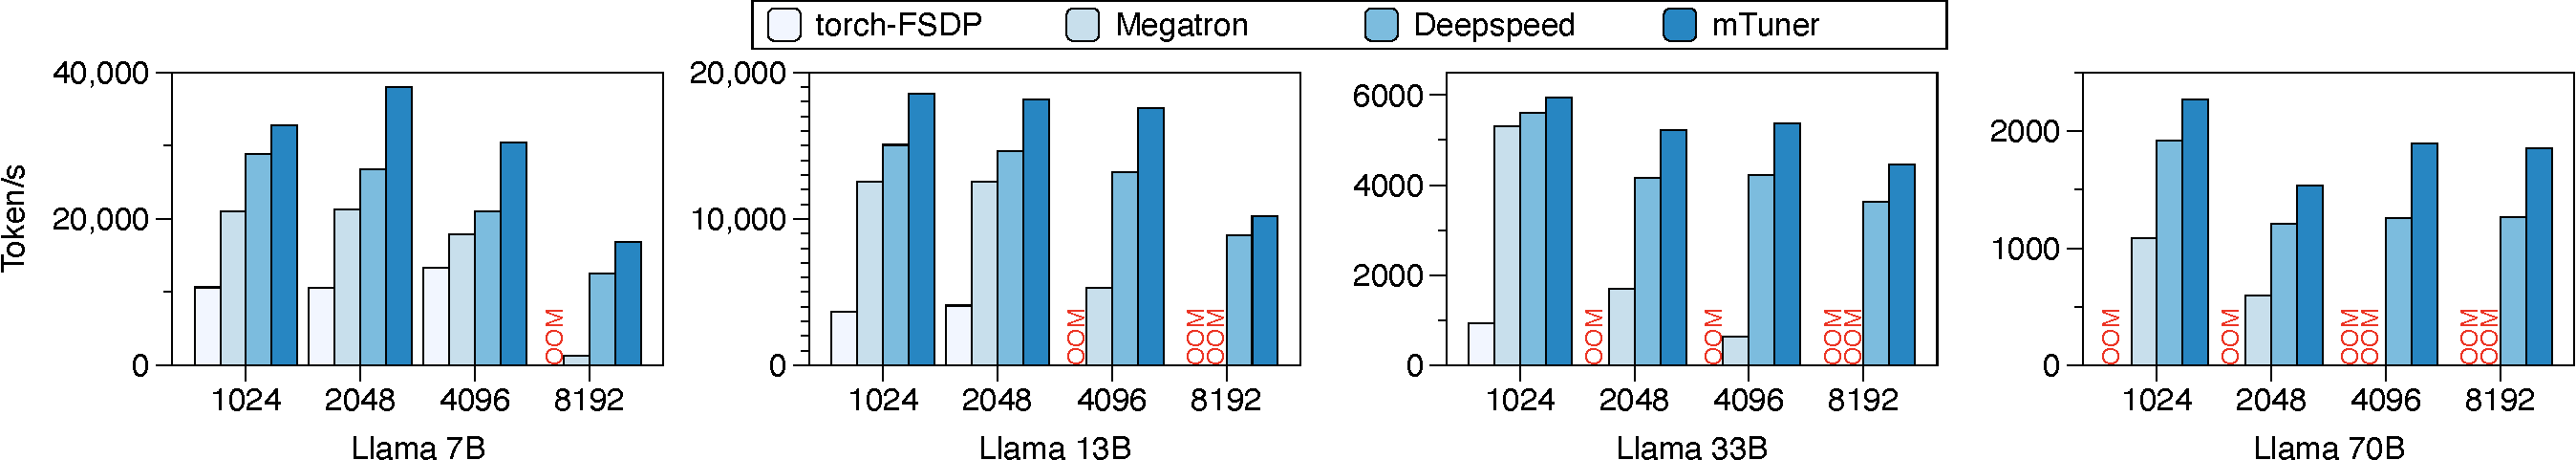
\includegraphics[width=\textwidth]{figures/mtuner/exp-img/overall-a100-crop.pdf}
         \caption{PCIe服务器}
         \label{fig:overall-a100}
     \end{subfigure}
     \vfill
     \begin{subfigure}[b]{\textwidth}
         \centering
         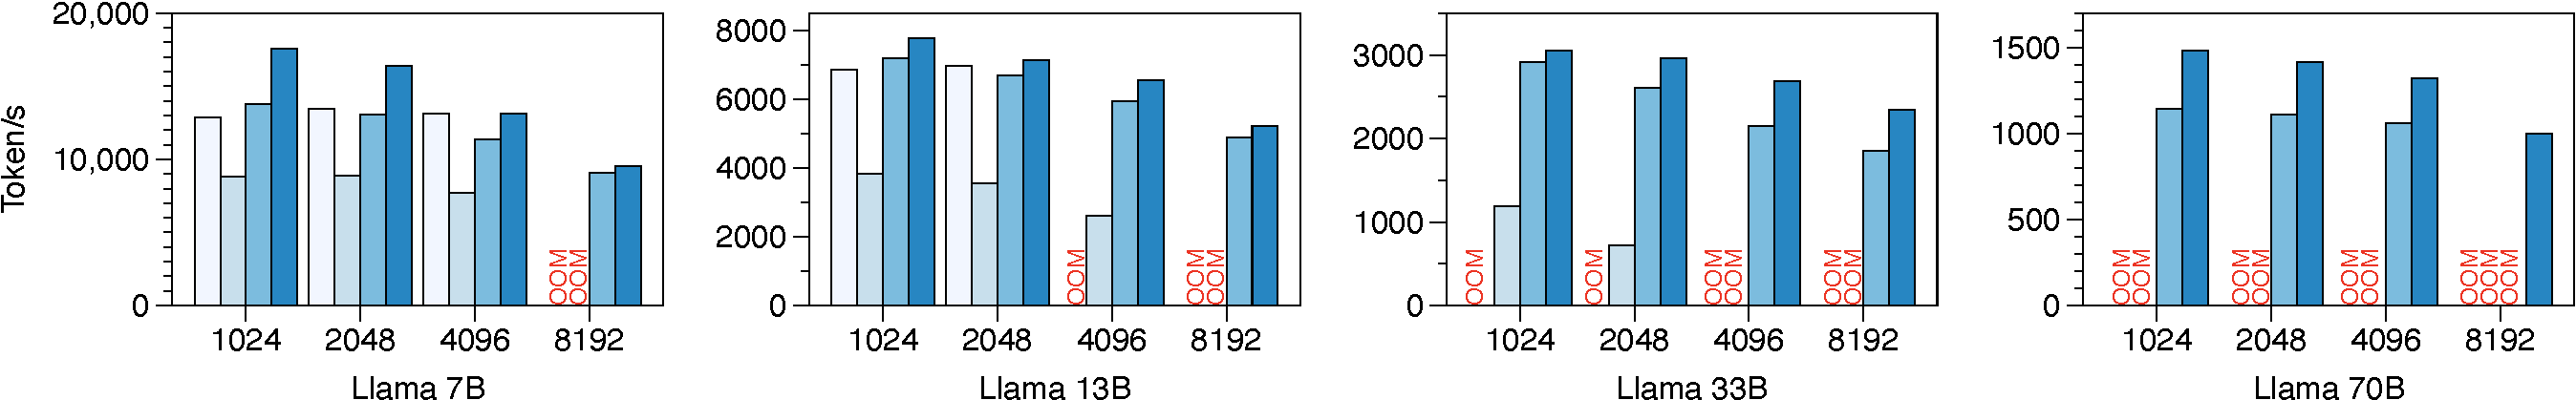
\includegraphics[width=\textwidth]{figures/mtuner/exp-img/overall-all-seq-v100-nvlink-crop.pdf}
         \caption{NVLink服务器}
         \label{fig:overall-v100}
     \end{subfigure}
     \caption{不同序列长度下的端到端性能}
     \label{fig:overall}
\end{figure*}


\subsection{端到端实验}

\Cref{fig:overall}展示了mTuner在不同模型、输入序列长度和硬件配置下的整体性能。  
\Cref{fig:overall-a100}展示了在PCIe服务器上的性能。  
DeepSpeed因为实现了高效的计算-通信重叠机制和通信算子,始终是基线方法中表现最好的。  
mTuner相比DeepSpeed可以将吞吐量提高28.3\%。
而相比于mTuner的实现基础Torch-FSDP,mTuner平均加速比达4.15倍。  
在如Llama-2-7B等较小的模型上,内存更为充足,mTuner可以充分利用可用内存,从而实现40\%的加速,并且吞吐量超过每秒30,000个词元。  
即使是在像33B和70B这样的大模型上,尽管模型参数本身就占据了大量内存,mTuner仍然实现了27\%的加速,这表明本研究提出的方法在各种模型规模下都具有良好的有效性。

本研究发现,对于具有更长序列长度的输入,mTuner更加有效。  
这是因为它们导致了更小的批次大小和更大的激活内存消耗,从而进一步增加了每个样本相对于权重的通信开销。  
在较长的序列(≥4096)情况下,mTuner实现了平均34\%的加速。

在比较PCIe服务器和NVLink服务器时,本研究发现mTuner在PCIe服务器配置下获得了更高的加速比(28.3\% vs. 15.5\%)。  
这主要原因是PCIe服务器上通信瓶颈更为严重,而mTuner通过增加内存利用率,恰好减少了通信开销,对整体性能的优化更显著。



\begin{figure}[ht]
     \centering
     \begin{subfigure}[b]{0.75\textwidth}
         \centering
         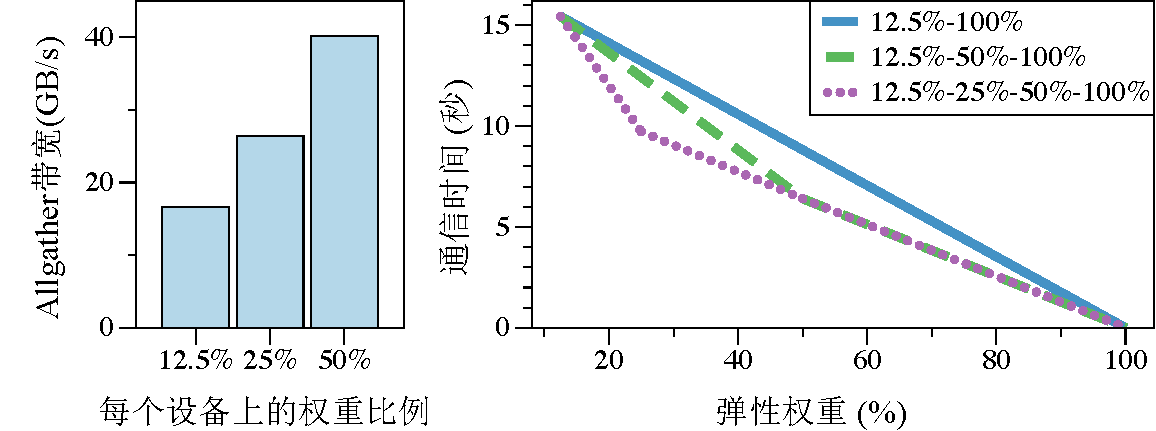
\includegraphics[width=\textwidth]{figures/mtuner/exp-img/weight-comm-pcie-crop.pdf}
         \caption{PCIe服务器}
         \label{fig:dp-change-1}
     \end{subfigure}
     \vfill
     \begin{subfigure}[b]{0.75\textwidth}
         \centering
         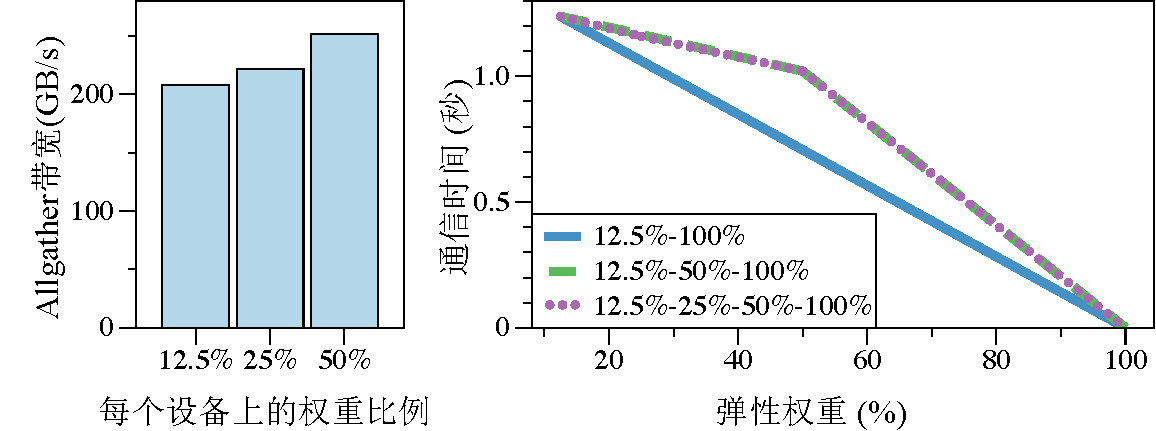
\includegraphics[width=\textwidth]{figures/mtuner/exp-img/weight-comm-nvlink-crop.pdf}
         \caption{NVLink服务器}
         \label{fig:dp-change-2}
    \end{subfigure}
        \caption{随着弹性权重比例增长的通信时间(在PCIe和NVLink服务器上)}
        \label{fig:dp-change}
\end{figure}

\subsection{弹性张量消融实验}

\Cref{fig:dp-change}展示了通过不同方式增加弹性权重比例所获得的结果。  
在相同内存使用的情况下,本研究观察到了不同的通信表现。  
不同颜色的线条代表在不同比例下优先增加弹性权重大小的情况。  
以\texttt{25\%-50\%-100\%}为例,它表示最初将某个算子的弹性权重比例从12.5\%增加到25\%(每块GPU最初存储12.5\%的权重)。  
随着权重的进一步增加,内存开销也随之增加,而通信时间则减少。  
当所有权重都增加到25\%后,继续将每个弹性权重的比例提升至50\%,随后再提升至100\%。  
当所有权重都增加到100\%时,所有权重都可在本地获取,通信时间为0。

如\Cref{fig:dp-change-1}所示,当总体权重大小小于25\%时,\texttt{25\%-50\%-100\%}的通信时间最少,因为它更好地利用了内存以提高通信效率。  
当总体弹性内存介于25\%和50\%之间时,\texttt{25\%-50\%-100\%}和\texttt{50\%-100\%}的性能趋于接近。  
至于\Cref{fig:dp-change-2}中的NVLink服务器,调度策略\texttt{100\%}直接避免了特定权重的通信,因此能够实现最佳的内存-通信曲线。  
其他两种调度策略仅在早期阶段减少了特定权重的通信工作负载,由于带宽相似,效果不如前者。

\begin{figure}[ht]
\centerline{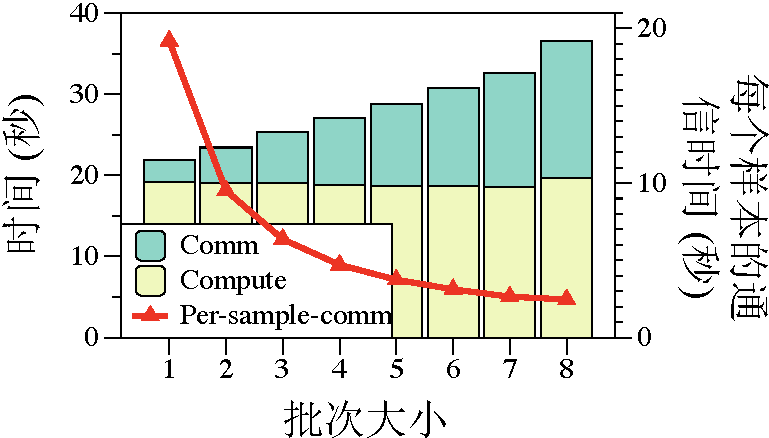
\includegraphics[width=0.42\textwidth]{figures/mtuner/exp-img/activation-comm-crop.pdf}}
\caption{不同批次大小对计算和通信时间的影响(在PCIe服务器上)}
\label{fig:eval-activation-comm}
\end{figure}

\Cref{fig:eval-activation-comm}展示了激活内存如何随着批次大小的变化影响计算与通信的效率。  
柱状图显示了在不同批次大小下,迭代过程中通信与计算的时间。  
本研究发现通信时间与批次大小无关,因为它仅与模型大小相关。  
因此,当增加批次大小时,分摊到每个样本的通信开销会减少。  
然而,计算时间与批次大小成正比,因为计算资源已达到饱和状态。

\begin{figure}[ht]
\centerline{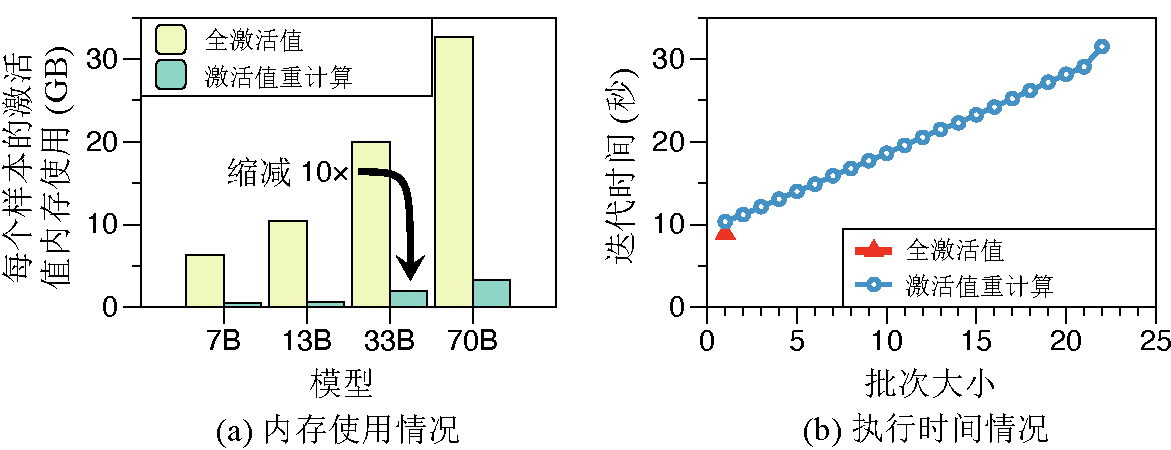
\includegraphics[width=0.73\textwidth]{figures/mtuner/exp-img/act-overhead-crop.pdf}}
\caption{不同模型的全部激活和检查点激活的对比(在PCIe服务器上)}
\label{fig:activation-overhead}
\end{figure}

\Cref{fig:activation-overhead}展示了激活检查点的效果及其开销。  
\Cref{fig:activation-overhead}(a)展示了在批量大小为1、序列长度为1024的情况下,所有生成的激活和检查点激活的内存消耗。  
对于不同规模的模型,mTuner可以将激活所需的内存减少10倍。  
这一减少对于Llama-2-70B尤为重要,因为保留所有激活需要超过30GB的设备内存。  
结合每个设备上权重的存储,这将导致内存溢出(OOM)错误,甚至无法支持批量大小为1的运行。

\Cref{fig:activation-overhead}(b)展示了激活检查点在Llama-2-33B上的引入开销。  
两种方法都可以在批量大小为1的情况下运行。  
然而,随着批量大小的增加,只有采用激活检查点的方法仍然可行。  
通过比较运行时间,激活检查点带来的重新计算开销非常小。  
这主要是因为执行时间主要由通信主导。  
而mTuner通过复用距离减轻了激活检查点带来的额外通信,从而降低了与激活检查点相关的运行时间开销。



\begin{figure}[ht]
\centerline{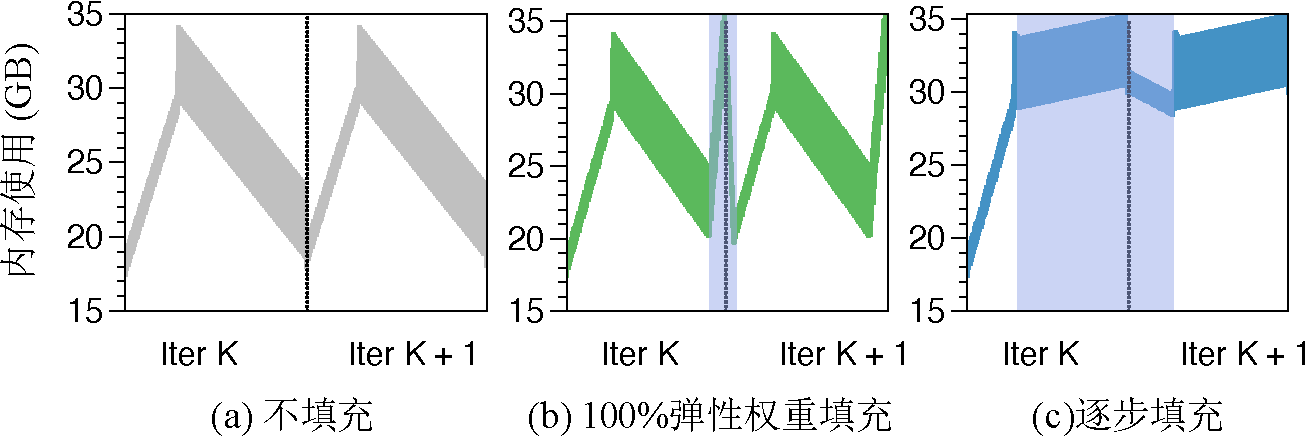
\includegraphics[width=0.75\textwidth]{figures/mtuner/exp-img/valley-reuse-crop.pdf}}
\caption{不同填充策略性下的内存-时间曲线}
\label{fig:eval-valley-reuse}
\end{figure}

\subsection{内存自适应执行计划消融实验}

\Cref{fig:eval-valley-reuse}展示了运行过程中内存变化的情况,每个子图代表两个迭代周期。  
从\Cref{fig:eval-valley-reuse}(a)可以看出,在每次迭代的前向传播阶段,内存使用持续增加,因为作为检查点的激活不断累积在内存中。  
而在反向传播阶段,内存呈锯齿状下降。  
这是因为在基于检查点进行重新计算时,前向传播过程中被丢弃的大量激活会被重新生成,而这些内存会在反向计算过程中立即被消耗。
从\Cref{fig:eval-valley-reuse}(b)可以看出,如果mTuner在谷值区域缓存并重复使用100\%的弹性权重,则谷值处的内存会迅速填满,导致只有少数算子的权重得到了优化,而大量的内存时间处于未充分利用状态。  
\Cref{fig:eval-valley-reuse}(c)表明,通过逐步填充谷值区域,大多数权重可以在较少通信的情况下增大尺寸,同时填满内存谷值区域。

\begin{figure}[ht]
\centerline{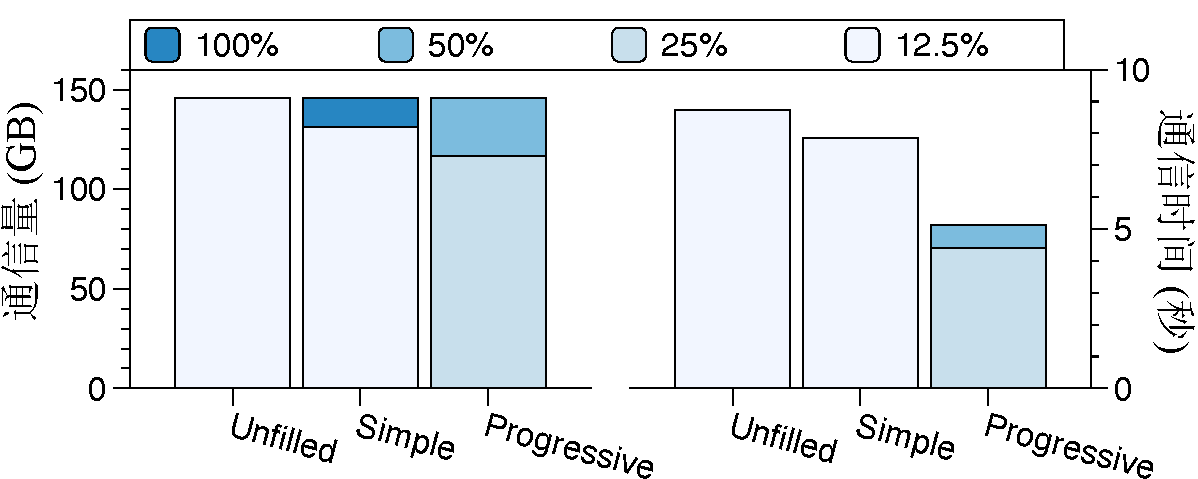
\includegraphics[width=0.6\textwidth]{figures/mtuner/exp-img/valley-effect-crop.pdf}}
\caption{弹性权重分布及相应的通信时间}
\label{fig:eval-valley-effect}
\end{figure}

\Cref{fig:eval-valley-effect}展示了这三种方法在前向传播阶段的弹性权重分布和通信时间。  
通信工作负载指的是收集的总权重,因此不同的填充方法(包括不填充)表现出相同的通信工作负载。  
本研究发现非渐进式填充方法仅有10.3\%的工作负载可以通过100\%的弹性权重进行通信,从而通过本地可用的权重减少10\%的整体通信时间。  
然而,通过使用渐进式方法填充谷值区域,80.2\%的权重可以通过25\%的弹性权重进行优化,其中有18.0\%的权重可以通过50\%的弹性权重进行优化,从而整体通信时间减少了41\%。

\begin{figure}[ht]
\centerline{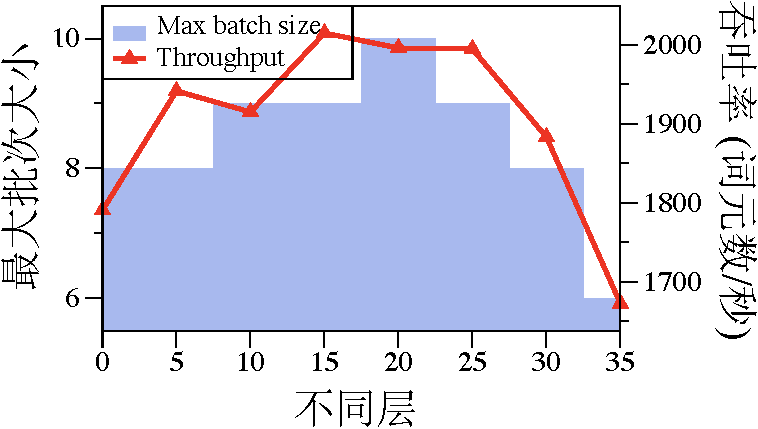
\includegraphics[width=0.45\textwidth]{figures/mtuner/exp-img/peak-crop.pdf}}
\caption{最大批处理大小及其对应的吞吐量随预峰值阶段层数变化情况}
\label{fig:eval-peak}
\end{figure}

\Cref{fig:eval-peak}展示了对于Llama-2-70B,mTuner可实现的最大批处理大小。  
通过调整预峰值阶段某些层的反向优先级并降低峰值高度,mTuner可以增加每次迭代的批处理大小。  
此外,为了减少在平坦峰值阶段小批量重复计算的开销,mTuner增加了平坦峰值部分的弹性权重比例。  
因此,当更多的层被展平时,内存开销也会增加,从而导致最大批处理大小下降。  
此外,由于平均通信工作负载与批处理大小相关,吞吐量在批处理大小达到最大值时也达到峰值,相比未展平峰值的情况,吞吐量提升了12\%。

\begin{figure}[ht]
\centerline{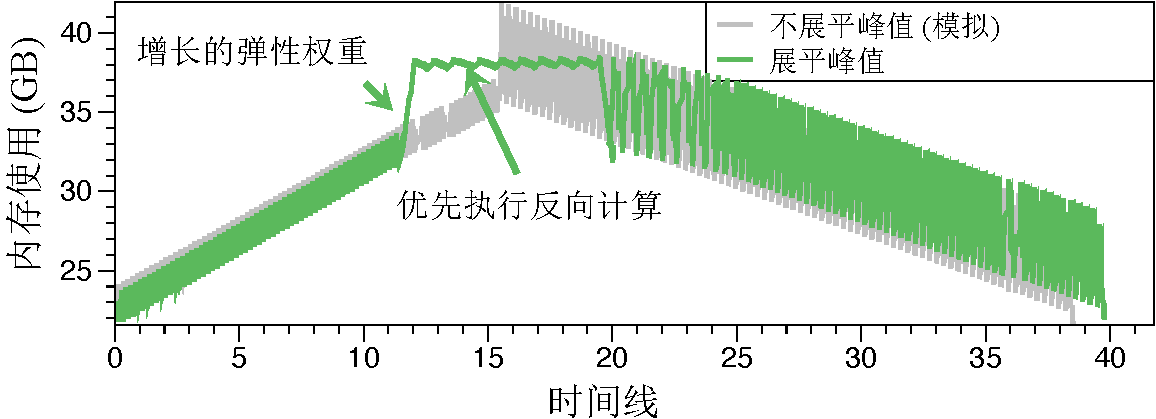
\includegraphics[width=0.7\textwidth]{figures/mtuner/exp-img/peak-flatten-crop.pdf}}
\caption{展平峰值前后的内存-时间曲线}
\label{fig:eval-flattened-peak}
\end{figure}

如\Cref{fig:eval-flattened-peak}所示,通过展平峰值可以有效降低内存峰值高度。  
为了减少展平峰值阶段重复执行带来的开销,mTuner在预峰值阶段增加了弹性权重大小,并在展平峰值结束时释放这些权重。  
然而,与模拟的正常执行相比,峰值展平仍然引入了一定的额外开销,导致执行时间略有增加(40秒 vs. 38秒)。  
但由峰值展平所带来的优势,例如更大的批处理大小和更低的每样本通信开销,仍然对整体性能产生了积极影响。

\subsection{示范应用}

\begin{figure}[ht]
\centerline{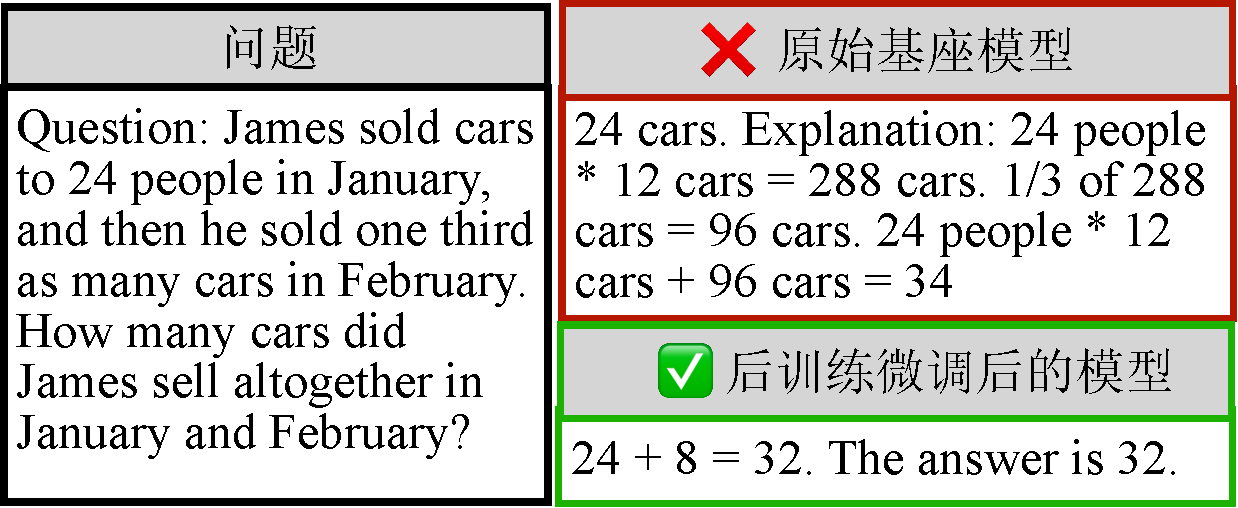
\includegraphics[width=0.55\textwidth]{figures/mtuner/exp-img/demo-crop.pdf}}
\caption{使用 mTuner 提升 Llama-2-13B 数学能力的示例}
\label{fig:eval-demo}
\end{figure}

\Cref{fig:eval-demo}展示了一个使用mTuner进行模型微调的示范应用案例。  
mTuner 使用来自数学数据集~\cite{math-datatset}的2亿个词元来提升Llama-2-13B的数学解题能力,仅用了3小时,模型就能针对数学问题生成正确且简洁的答案。

% \subsection{性能比较}
% 图 7 展示了 mTuner 与 Deepspeed 和 Megatron 在不同模型规模上的吞吐量比较。结果表明,mTuner 在所有模型规模上都显著优于 Deepspeed 和 Megatron。在 7B 模型上,mTuner 的吞吐量比 Deepspeed 高 1.23 倍,比 Megatron 高 1.18 倍。在 13B 模型上,mTuner 的吞吐量比 Deepspeed 高 1.35 倍,比 Megatron 高 1.27 倍。在 30B 模型上,mTuner 的吞吐量比 Deepspeed 高 1.42 倍,比 Megatron 高 1.34 倍。在 70B 模型上,mTuner 的吞吐量比 Deepspeed 高 1.51 倍,比 Megatron 高 1.45 倍。平均而言,mTuner 的吞吐量比 Deepspeed 高 1.28 倍,比 Megatron 高 1.22 倍。
% 这些结果表明,mTuner 能够有效地利用弹性张量来优化内存使用和减少通信开销,从而显著提高微调性能。通过动态调整权重和激活的内存使用量,mTuner 能够更好地适应不同模型规模和内存状态,实现更高的训练效率。
% \subsection{内存使用分析}
% 图 8 展示了 mTuner 与 Deepspeed 和 Megatron 在 13B 模型上的内存使用情况比较。结果表明,mTuner 能够更有效地利用内存。在峰值内存使用方面,mTuner 比 Deepspeed 低 23\%,比 Megatron 低 18\%。这是因为 mTuner 通过调整批次大小和采用激活重计算技术,降低了激活的峰值内存使用量。在平均内存使用方面,mTuner 比 Deepspeed 高 12\%,比 Megatron 高 8\%。这是因为 mTuner 在内存相对充裕时,通过增加弹性权重大小来减少通信量,从而提高了内存利用率。
% 这些结果表明,mTuner 在内存管理方面具有优势。通过灵活调整权重和激活的内存使用量,mTuner 能够在保证不超过设备内存限制的前提下,充分利用空闲内存,提高内存利用率,同时降低峰值内存使用量,避免内存不足的问题。
% \subsection{特定领域微调}
% 本章还评估了 mTuner 在特定领域微调任务中的性能。本章使用 Llama-2 13B 模型在数学数据集 [12] 上进行微调,以增强其数学能力。图 9 展示了 mTuner 与 Deepspeed 和 Megatron 在数学数据集上的微调时间比较。结果表明,mTuner 能够显著缩短微调时间。mTuner 在 3 小时内完成了微调,而 Deepspeed 需要 4.5 小时,Megatron 需要 5 小时。
% 这些结果表明,mTuner 不仅在通用语言任务的微调中表现出色,而且在特定领域任务的微调中也具有显著优势。通过提高微调性能,mTuner 能够更快地使模型适应特定领域,提高模型在特定领域任务中的表现。


\section{结论}
本章提出了一个利用弹性张量在多 GPU 服务器上加速参数高效微调的系统 mTuner。
通过对后训练 PEFT 微调中内存使用情况的详细分析,发现权重和激活的内存都可以进行动态连续的调整。
基于此观察,提出了弹性张量的概念,使张量的大小能够在运行时动态灵活地改变,从而提高内存利用率。
进一步,基于弹性张量构建了 mTuner,它能够感知内存状态并制定内存自适应执行计划。
实验结果表明,与最先进的训练系统相比,mTuner 在各种规模的大语言模型上实现了显著的性能提升,吞吐量最高提升可达 1.51 倍(平均提升 1.28 倍)。
mTuner 还能够在 3 小时内对 Llama-2-13B 模型进行微调,实现数学能力的增强。
% 未来,计划进一步探索如何将 mTuner 应用于更广泛的模型和任务,并研究如何在不同的硬件平台上优化 mTuner 的性能,还将研究如何将 mTuner 与其他先进的训练技术相结合,以进一步提高微调效率。

% \section{论文的语言及表述}

% 除国际研究生外,学位论文一律须用汉语书写。
% 学位论文应当用规范汉字进行撰写,除古汉语研究中涉及的古文字和参考文献中引用的外文文献之外,均采用简体汉字撰写。

% 国际研究生一般应以中文或英文书写学位论文,格式要求同上。
% 论文须用中文封面。

% 研究生学位论文是学术作品,因此其表述要严谨简明,重点突出,专业常识应简写或不写,做到立论正确、数据可靠、说明透彻、推理严谨、文字凝练、层次分明,避免使用文学性质的或带感情色彩的非学术性语言。

% 论文中如出现一个非通用性的新名词、新术语或新概念,需随即解释清楚。



% \section{论文题目的写法}

% 论文题目应简明扼要地反映论文工作的主要内容,力求精炼、准确,切忌笼统。
% 论文题目是对研究对象的准确、具体描述,一般要在一定程度上体现研究结论,因此,论文题目不仅应告诉读者这本论文研究了什么问题,更要告诉读者这个研究得出的结论。
% 例如:“在事实与虚构之间:梅乐、卡彭特、沃尔夫的新闻观”就比“三个美国作家的新闻观研究”更专业、更准确。



% \section{摘要的写法}

% 论文摘要是对论文研究内容的高度概括,应具有独立性和自含性,即应是 一篇简短但意义完整的文章。
% 通过阅读论文摘要,读者应该能够对论文的研究 方法及结论有一个整体性的了解,因此摘要的写法应力求精确简明。
% 论文摘要 应包括对问题及研究目的的描述、对使用的方法和研究过程进行的简要介绍、 对研究结论的高度凝练等,重点是结果和结论。

% 论文摘要切忌写成全文的提纲,尤其要避免“第 1 章……;第 2 章……;……”这样的陈述方式。



% \section{引言的写法}

% 一篇学位论文的引言大致包含如下几个部分:
% 1、问题的提出;
% 2、选题背 景及意义;
% 3、文献综述;
% 4、研究方法;
% 5、论文结构安排。
% \begin{itemize}
%   \item 问题的提出:要清晰地阐述所要研究的问题“是什么”。
%     \footnote{选题时切记要有“问题意识”,不要选不是问题的问题来研究。}
%   \item 选题背景及意义:论述清楚为什么选择这个题目来研究,即阐述该研究对学科发展的贡献、对国计民生的理论与现实意义等。
%   \item 文献综述:对本研究主题范围内的文献进行详尽的综合述评,“述”的同时一定要有“评”,指出现有研究状态,仍存在哪些尚待解决的问题,讲出自己的研究有哪些探索性内容。
%   \item 研究方法:讲清论文所使用的学术研究方法。
%   \item 论文结构安排:介绍本论文的写作结构安排。
% \end{itemize}



% \section{正文的写法}

% 本部分是论文作者的研究内容,不能将他人研究成果不加区分地掺和进来。
% 已经在引言的文献综述部分讲过的内容,这里不需要再重复。
% 各章之间要存在有机联系,符合逻辑顺序。



% \section{结论的写法}

% 结论是对论文主要研究结果、论点的提炼与概括,应精炼、准确、完整,使读者看后能全面了解论文的意义、目的和工作内容。
% 结论是最终的、总体的结论,不是正文各章小结的简单重复。
% 结论应包括论文的核心观点,主要阐述作者的创造性工作及所取得的研究成果在本领域中的地位、作用和意义,交代研究工作的局限,提出未来工作的意见或建议。
% 同时,要严格区分自己取得的成果与指导教师及他人的学术成果。

% 在评价自己的研究工作成果时,要实事求是,除非有足够的证据表明自己的研究是“首次”、“领先”、“填补空白”的,否则应避免使用这些或类似词语。
